
\begin{figure}
\begin{center}
    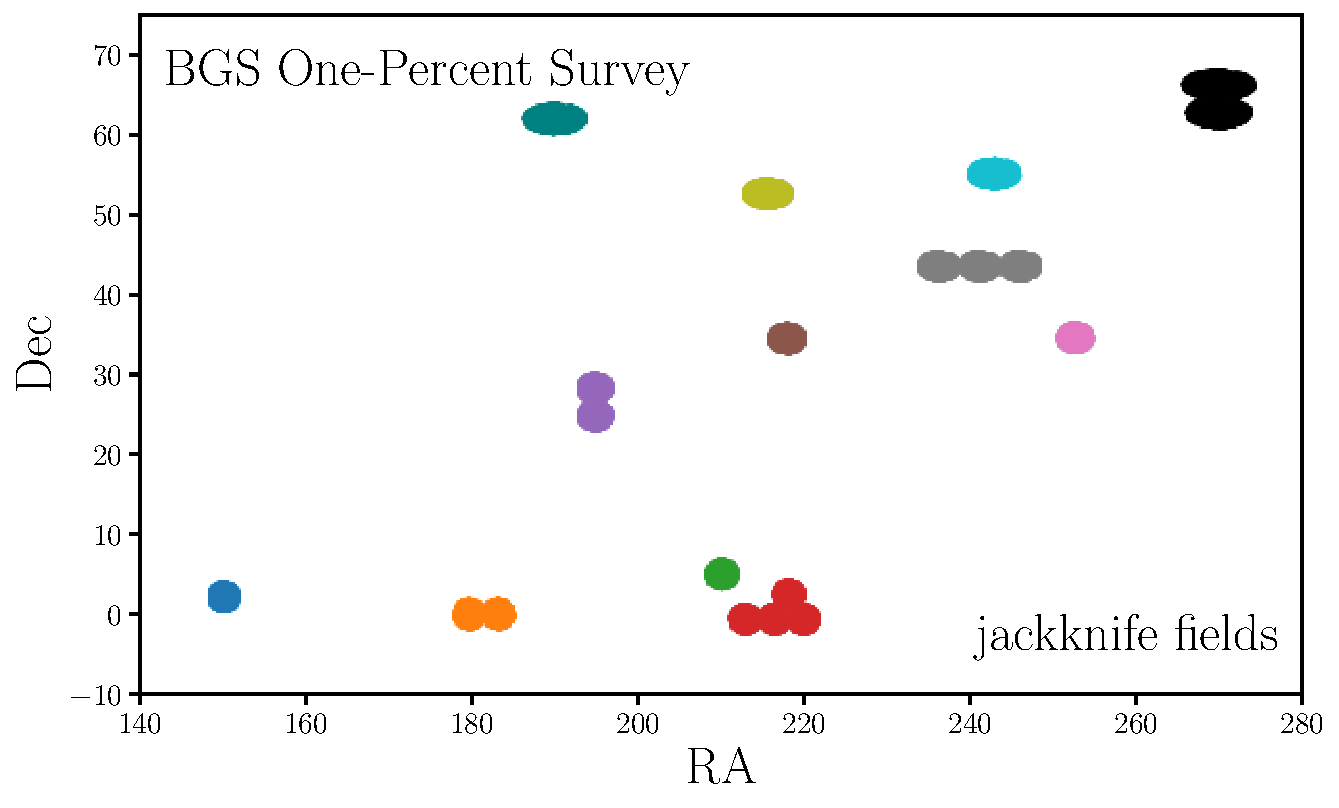
\includegraphics[width=0.5\textwidth]{figs/jackknife_fields.pdf} 
    \caption{
        The RA and Dec of the 12 jackknife fields of the BGS One-Percent Survey
        used to estimate the uncertainties on the SMF from sample variance. 
        We mark each field with a distinct color. 
    }\label{fig:jack}
\end{center}
\end{figure}


\section{Uncertainties on the SMF} \label{sec:jack}
We estimate the uncertainties of the SMF from sample variance using the
standard jackknife technique. 
This involves splitting our BGS sample into subsamples and then estimating
uncertainties using the subsample-to-subsample variations:  
\begin{equation} \label{eq:jack} 
    \sigma_\Phi = \left(\frac{N_{\rm jack}-1}{N_{\rm jack}}
    \sum\limits_{k=1}^{N_{\rm jack}} (\Phi_k - \Phi)^2 \right).
\end{equation} 
$N_{\rm jack}$ is the number of jackknife subsamples and $\Phi_k$ represents
the SMF estimated from the BGS galaxies excluding the jackknife subample $k$. 
In this work, we split the BGS sample into 12 jackknife fields based on the
angular positions of galaxies. 
We present the jackknife fields in Figure~\ref{fig:jack} with distinct colors. 
